%% +++++++++++++++++++++++++++++++++
%% Setzen von scrreprt
%% +++++++++++++++++++++++++++++++++
\documentclass[
11pt,
titlepage,
a4paper,
abstracton,
twoside,
openright,
chapterprefix,
noappendixprefix,
headsepline,
footsepline,
cleardoubleplain,
bibtotoc,
liststotoc,
pointlessnumbers
]{scrreprt}

%% +++++++++++++++++++++++++++++++++
%% Einbinden von Paketen
%% +++++++++++++++++++++++++++++++++
\usepackage{istitle}
\usepackage{geometry}
\usepackage[utf8]{inputenc} 
\usepackage[T1]{fontenc}
\usepackage{ae,aecompl}
\usepackage{amsmath}
\usepackage{amsthm}
\usepackage{amscd}
\usepackage{amsfonts}
\usepackage{amssymb}
\usepackage{listings}
\usepackage{xcolor}
\usepackage[german,ngerman]{babel}
\usepackage{graphicx}
\usepackage{url}
\usepackage[automark]{scrpage2}
%\usepackage{natbib}
\usepackage{bbm}
\usepackage{array}
\usepackage{booktabs}
\usepackage{threeparttable}
\usepackage{pifont}
\usepackage{placeins}
\usepackage[font=small,labelfont=bf,labelsep=colon]{caption}

% Settings for generating the PDF
% See https://www.tug.org/applications/hyperref/manual.html

\usepackage{hyperref}

\hypersetup{
	pdfinfo={ 
    		Title={Diplomarbeit},
		Creator={TeX},
		Producer={pdfTeX 0.15a},
		Author={},
		CreationDate={D:20091004000000},
		ModDate={D:20130331000000},
		Subject={Master thesis},
		Keywords={}
	},
	pdfpagelayout=TwoColumnRight,
	pdfdisplaydoctitle=true
}



%\input{linkcolors-pdf} % Links klickbar, vom PDF-Viewer hervorgehoben
%\input{linkcolors-colored} % Links klickbar, farbig hervorgehoben
\input{linkcolors-print} % Links klickbar, aber nicht hervorgehoben



%% +++++++++++++++++++++++++++++++++
%% Header
%% +++++++++++++++++++++++++++++++++

% Seitengeometrie
\geometry{a4paper,outer=38mm,inner=26mm,top=40mm,bottom=50mm}

% Definition von arg max
\DeclareMathOperator*{\argmax}{arg\,max}

% Definition von Sternchen
\newcommand{\sig}{\ding{73}}
\newcommand{\ssig}{\ding{72}}

% Definition von Häkchen und Kreuzchen
\newcommand{\h}{\ding{51}}
\newcommand{\x}{\ding{55}}

% Farben definieren
\definecolor{lightgrey}{rgb}{0.99,0.99,0.99}
\definecolor{colKeys}{rgb}{0,0,1}
\definecolor{colIdentifier}{rgb}{0,0,0}
\definecolor{colComments}{rgb}{1,0,0}
\definecolor{colString}{rgb}{0,0.5,0}

\definecolor{darkred}{rgb}{0.5,0,0}
\definecolor{darkgreen}{rgb}{0,0.5,0}
\definecolor{darkblue}{rgb}{0,0,0.5}
\definecolor{green}{rgb}{0,0.7,0}
\definecolor{blue}{rgb}{0,0,0.7}
\definecolor{red}{rgb}{0.7,0,0}
\definecolor{black}{rgb}{0,0,0}

% Quellcode
\lstloadlanguages{XML} 
\lstset{
    float=hbp,
    keywordstyle=\color{colKeys},
    stringstyle=\color{colString},
    commentstyle=\color{colComments},
    basicstyle=\texttt\small,
    identifierstyle=\color{colIdentifier},
    columns=flexible,
    tabsize=2,
    frame=single,
    extendedchars=true,
    showspaces=false,
    showstringspaces=false,
    numbers=none,
    numberstyle=\tiny,
    breaklines=true,
    backgroundcolor=\color{lightgrey},
    breakautoindent=true,
	captionpos=b,
	xleftmargin=\fboxsep,
	xrightmargin=\fboxsep,
	frameround=tttt,
	inputencoding=utf8,
	extendedchars=true,
	literate={ä}{{\"a}}1 {ü}{{\"u}}1 {ö}{{\"o}}1,
}

% Kopf- und Fußzeilen
\pagestyle{scrheadings}
\ihead[]{}
\chead[]{}
\ohead[]{\textsf{\headmark}}
%\ifoot[]{}
%\cfoot[]{}
%\ofoot[]{\textsf{\pagemark}}

% Absätze
\setlength{\parindent}{0pt}
\setlength{\parskip}{2ex}

\def\topfraction{1.0} 
\def\bottomfraction{1.0} 
\def\textfraction{0.0}

\renewcommand*{\partpagestyle}{empty}

% Überschrift des Abstracts
\addto\captionsngerman{\renewcommand*\abstractname{Kurzzusammenfassung}}
% Überschrift des Verzeichnisses der Listings
\addto\captionsngerman{\renewcommand*\lstlistlistingname{Auflistungsverzeichnis}}
% Name von Listings
\addto\captionsngerman{\renewcommand*\lstlistingname{Auflistung}}


%% +++++++++++++++++++++++++++++++++
%% Start des Dokuments
%% +++++++++++++++++++++++++++++++++
\begin{document}

% Titelseite
\title{Extraktion von Entitäten aus Suchergebnissseiten}
\author{Denis Repkov}
\tutor{Professor~Dr.-Ing.~Norbert Fuhr}
{Dipl.-Inform.~Sebastian Dungs}
\thesistype{Masterarbeit}

\logo{Bilder/logo_uni.png}
\timeperiod{Mai 2015}{November 2015}
\pagenumbering{alph}
\maketitle

% Kurzzusammenfassung (Abstract)
\setcounter{page}{2}
\begin{abstract}
\thispagestyle{plain}
Im Rahmen dieser Arbeit wird eine neue Möglichkeit von Benutzerunterstützung bei der Websuche erforscht, die dem Benutzer einen Übersicht über in den Suchergebnissen vorhandene Entitäten wie Personen, Firmen, Städte oder Länder, liefert. Es wird eine Erweiterung für das Stanbol-NLP-Framework entwickelt, die verschiedene NER\footnote{Named Entity Extraktion - Extraktion von Entitäten}-Algorithmen implementiert. Zusätzlich dazu wird eine API aufgebaut, die dem Entwickler, der keine Vorwissen über NLP\footnote{Natural Language Processing - Natürlichsprachliche Mensch-Computer-Interaktion} besitzt, die Möglichkeit gibt, die Extraktion von Entitäten in eine beliebige Suchapplikation zu integrieren. 

Die vorliegende Arbeit ist auf deutschsprachige Webseiten orientiert, aber die Grundprinzipien lassen sich auch auf andere Sprachen erweitern.

Anschließend durchgeführte Evaluierung zeigt, dass das entwickelte System tatsächlich für die Benutzerunterstützung verwendet werden könnte, obwohl die graphische Oberfläche des Systems noch angepasst werden muss. Es wird außerdem gezeigt, dass es wichtig ist, dass die Suchergebnisse nicht mit allen gefundenen Entitäten angereichert werden, sondern nur mit den Entitäten, die als ,,wichtig`` eingestuft wurden. Als Maß für die ,,Wichtigkeit`` einer Entität werden in dieser Arbeit die Gewichte, die direkt von Extraktionsalgorithmen bestimmt werden, verwendet. Es wird aber gezeigt, dass solches Maß Nachteile hat, und dass die ,,Wichtigkeit`` einer Entität in den zukünftigen Arbeiten für jeden Benutzer personalisiert definiert werden soll.
\end{abstract}

% Inhaltsverzeichnis
\pagestyle{scrheadings}
\setcounter{tocdepth}{2}
\tableofcontents

% Text
\cleardoublepage
\pagenumbering{arabic}
\pagestyle{scrheadings}
\sloppy
\chapter{Einleitung}
Im Abschnitt \ref{sec:Motivation} wird die Motivation zu dieser Arbeit
erläutert. Darauffolgend (\ref{sec:Aufgabenstellung}) wird die Aufgabenstellung
beschrieben. Abschließend gibt Abschnitt \ref{sec:Aufbau der Arbeit} einen Überblick über
den Aufbau der Arbeit.

\section{Motivation}
\label{sec:Motivation}


\section{Aufgabenstellung}
\label{sec:Aufgabenstellung}


\section{Aufbau der Arbeit}
\label{sec:Aufbau der Arbeit}
\chapter{Grundlagen}

\section{Extraktion von Entitäten} \label{sec:Grundlagen}
\paragraph{}
%Was sind die Entitäten - kurze Einleitung. Wie genau können die Entitäten aus einem Text extrahiert werden? Welche Einsätze gibt es? Wofür kann man Entitäten verwenden?
Vijay Krishnan hat in seiner Arbeit\cite{Vijay/Vignesh:05} die Extraktion von Entitäten als Suche nach atomaren Elementen im Text und ihre Zuordnung bestimmten vordefinierten Klassen wie Person, Organisation, geographische Lokation usw. definiert. Zum Beispiel betrachten wir folgenden Text aus Wikipedia: ,,Seit dem 1. Januar 2014 ist Bill de Blasio neuer Bürgermeister von New York.``. Dabei soll das Framework, das die Entitäten aus dem Text extrahiert, die Entität \textit{Bill de Blasio} als eine Person erkennen, die Entität \textit{New York} als ein geographisches Objekt, und \textit{1. Januar 2014} als ein Datum.

\paragraph{}
Es stellt sich die Frage, wie genau die Entitäten für die Benutzerunterstützung bei der Suche eingesetzt werden können. Wenn die einzige Informationen, die dem Benutzer zur Verfügung stehen würde, nur der Name, die Klasse und Position der Entität innerhalb des Textes wären, wären Entitäten kaum verwendbar. Aber wenn jeder Entität eine Menge von Eigenschaften (wie Geburtsdatum für eine Person) und Verbindungen zu anderen Entitäten (Z.b. Geburtsort einer Person könnte ein Link auf eine geografische Entität sein) zugeordnet wird, könnte der Benutzer theoretisch die aus der Entität gewonnene Informationen für Präzisierung der Suchanfrage verwenden.

\paragraph{}
Aber wie könnten die Entitäten aus einem natürlichsprachlichen Text extrahiert werden? Die einfachste Möglichkeit wäre der Einsatz von ,,fest definierten`` Regeln, die dann auf den ganzen Text angewendet werden, und entscheiden, ob das nächste Wort eine Entität ist oder nicht. Dieser Einsatz soll in dieser Arbeit aber nicht eingesetzt werden, da er folgende Nachteile\cite{baluja2000applying} hat:
\begin{enumerate}
\item So ein ,,festes`` System ist nicht in der Lage, Änderungen automatisch zu 'erlernen' und muss für jede Änderung neu angepasst/programmiert werden.
\item Derartige ,,feste`` Systeme neigen dazu, mit der Zeit sehr komplex zu werden, und ab irgendeinem Zeitpunkt wird die Anpassung von Regeln unmöglich beziehungsweise mit einem großen technischem Aufwand verbunden sein.
\item Solche Systeme können nicht wirklich gut mit den fehlerhaften Daten wie Schreibfehler arbeiten, was im Fall von Websuche sehr oft auftreten kann.
\end{enumerate}  
Der einzige Vorteil von solchen festen Systemen ist dass die für sehr kleine Domäne eventuell gut funktionieren können, was allerdings für Websuche nicht ausreichend ist.

Aber welche Methode ist für die Extraktion von Entitäten passend? Wie erwähnt, gehört jede Entität irgendeiner Klasse. Deswegen kann man die Extraktion von Entitäten als Klassifikationsaufgabe definieren, und die Methoden des maschinellen Lernens, die man für die Klassifizierung anwendet, einsetzen, wie es z.B. in der Arbeit von William Cohen\cite{cohen2004exploiting} beschrieben wurde. In dieser Arbeit werden drei verschiedene Einsätze verglichen und eingesetzt: \textbf{Conditional Random Field}, \textbf{Support Vector Machines} und \textbf{Maximum Entropy}.

\subsection{Features}
\paragraph{}
Wie für jede andere Klassifizierungsaufgabe müssen für die Extraktion von Entitäten die Parameter definiert werden, die jedes zu klassifizierendes Objekt beschreiben. Im Fall von Extraktion von Entitäten  heißt das, dass jedem Wort ein Vektor von Eigenschaften zugeordnet werden muss. Nadeau\cite{nadeau2007survey} hat die Eigenschaften, die ein Wort haben kann, in drei Gruppen geteilt:

\begin{itemize}
\item Boolesche Eigenschaften wie ,,Ob das Wort groß geschrieben wird``.
\item Numerische Eigenschaften wie die Länge des Wortes.
\item Nominale Eigenschaften wie Präfix oder Suffix.
\end{itemize}
Zusätzlich dazu wurde von Hai\cite{chieu2002named} die Verteilung in lokale und globale Eigenschaften vorgeschlagen:

\begin{enumerate}
\item Globale Eigenschaften:
\begin{enumerate}
\item Personenpräfixe für bestimmtes Wort in anderen Sätzen des Dokumentes: z.B. wenn wir im Text zuerst die Tokens ,,Frau Sony`` treffen, und dann einfach ,,Sony``, dann soll angenommen werden, dass ,,Sony`` eine Entität der Klasse ,,Person`` ist.
\item Abkürzungen: wenn in einem Satz mehr Wörter nacheinander groß geschrieben werden, wie z.B. ,,Deutsche Demokratische Republik``, dann wird in dem Text nach entsprechender Abkürzung gesucht: ,,DDR``, und wenn Abkürzung eine Entität ist, können auch alle entsprechende Tokens als eine Entität markiert werden.
\end{enumerate}
\item Lokale Eigenschaften:
\begin{enumerate}
\item Ob das Wort groß geschrieben wird.
\item Ob vorheriges oder nächstes Wort großgeschrieben wird.
\item Ob alle Zeichen im Wort großgeschrieben werden.
\item Ob es ein Punkt am Ende des Wortes steht.
\item Ob das Wort Zahlen beinhaltet, und falls ja, wie viel.
\item Ob das Wort das Prozent- oder Dollarzeichen beinhaltet.
\item Bestimmte Hilfswörter (wie ,,Frau`` oder ,,GmbH``), die entweder vor oder nach dem Wort, das untersucht werden muss, stehen.
\item Ob das Wort nur aus Zahlen besteht.
\item POS-Tag des Wortes (ob das Wort ein Substantiv oder ein Verb ist)
\item POS-Tags der Wörter, die vor dem ausgewählten Wort stehen.
\end{enumerate}
\end{enumerate}
Dabei beschreiben lokale Features die Eigenschaften, die nur die Informationen, die aus dem Wort selbst und aus den benachbarten Wörtern in demselben Satz gewonnen werden können, brauchen. Globale Eigenschaften benutzen dagegen auch die Vorkommnisse vom Wort im ganzen Dokument.

Das oben genannte Features werden ,,supervised Features`` genannt, weil die von einem Mensch bestimmt wurden. Zusätzlich dazu wird in der Arbeit von Turian\cite{turian2010word} der Einsatz von sogenannten ,,unsupervised Features`` vorgeschlagen, die während des Lernvorganges berechnet werden. Es wird in der zitierten Arbeit zwischen folgenden Gruppen von ,,unsupervised Features`` unterschieden:
\begin{enumerate}
\item Distributional Features - eine Matrix der Größe $W \times C$, wo $W$ die Anzahl von Wörtern im Wörterbuch beschreibt und $C$ die Anzahl von verschiedenen Kontexten.
\item Auf Cluster basierte Features - es wird versucht, die Wörter automatisch in Clusters zu teilen.
\item Word Embedding - Dieses Modell wird hauptsächlich in den neuronalen Modellen eingesetzt, und erlernt Eigenschaften aus N-Grammen, mithilfe von Lookup-Tabellen.
\end{enumerate}

\paragraph{}
Der Vorgang zum Aufbau eines ,,Distributional Features``-Modells wurde in der Arbeit von Sahlgren\cite{sahlgren2006word} beschrieben. Als Basisdatenstruktur wird die Co-occurence-Matrix verwendet, die beschreibt, welche Wörter zusammen in einem Context gesehen werden. Die Anzahl von Zeilen und Spalten in dieser Matrix ist dabei der Anzahl von Wörtern im zu analysierenden Korpus gleich. Ein Beispiel solcher Matrix für den Satz ,,Leela mag dramatische Filme und Bücher`` finde man in der Abbildung \ref{fig:COOC-MAT}

\begin{figure}[ht]
\setbox0\vbox{\small}
$$
\begin{array}{ccccccc}
 & Leela & mag & dramatische & Filme & und & B\ddot{u}cher \\ 
Leela & 0 & 1 & 0 & 0 & 0 & 0 \\ 
mag & 1 & 0 & 1 & 0 & 0 & 0 \\ 
dramatische & 0 & 1 & 0 & 1 & 0 & 0 \\ 
Filme & 0 & 0 & 1 & 0 & 1 & 0 \\ 
und & 0 & 0 & 0 & 1 & 0 & 1 \\ 
B\ddot{u}cher & 0 & 0 & 0 & 0 & 1 & 0
\end{array} 
$$
\caption{Beispiel einer Co-occurence-Matrix}
\label{fig:COOC-MAT}
\end{figure}

Aus dieser Matrix soll für jedes Wort ein Vektor aufgebaut werden, der die Lage des Wortes in einem $n$-dimensionalen Raum beschreibt. Dieser Vektor kann später für die Berechnung vom Abstand zwischen Wörtern verwendet werden, was in den späteren Schritten als Maße für ,,Gleichheit`` von Wörtern verwendet werden kann.

\paragraph{}
Ein Beispiel für auf Cluster basierte Features wäre Brown-Algorithmus\cite{sun2011semi}. Dieses Algorithmus funktioniert auf folgende Art und Weise:
\begin{enumerate}
\item Zuerst wird jedem Wort eine eigene Klasse zugeordnet
\item Die Clusters werden paarweise iterativ zusammengefügt.
\item Dabei werden die Zwischenschritte der Clusterisierung gespeichert, so dass man am Ende alle Schritte nachverfolgen kann, und ein binäres Baum aufbauen könnte, wo jeder Endknoten ein Wort darstellt.  
\end{enumerate}

Eine graphische Darstellung des Brown-Algorithmus findet man auf der Abbildung \ref{fig:BROWN-CLUSTER}.

\begin{figure}[ht]
\setbox0\vbox{\small}
\begin{tikzpicture}[>=Stealth]
\graph[binary tree layout]{
  ROOT -> {   
    C1 -> { 
      C12 -> { 
        C123 -> { Wort1, Wort2 },
        Wort9
      }, 
    C2 -> { Wort3, Wort4 }
    },
      C3 -> {
        C31 -> { Wort5, Wort6 },
        C32 -> { Wort7, Wort8 }
      }
  }
};
\end{tikzpicture}
\caption{Brown-Algorithmus}
\label{fig:BROWN-CLUSTER}
\end{figure}

\paragraph{}
Ein sehr interessanter Einsatz fürs ,,Word Embedding`` wird in der Arbeit von Xin\cite{rong2014word2vec} ausführlich erklärt. Wie in ,,Distributional Features``-Modellen wird für die Wörter ein Vektor berechnet, und geometrischer Abstand zwischen zwei Punkten im Feature-Raum bestimmt die Ähnlichkeit von Wörtern, zusätzlich dazu kann auch die Ausrichtung des Vektors im Kauf genommen werden. Die entsprechende Vektoren werden mit Hilfe eines neuronales Netzes berechnet, das auf zwei verschiedene Art und Weisen implementiert werden kann: \textit{CBOW} und \textit{Skip-gram}\cite{wang2014introduction}:

Die erste Methode - CBOW (Continuous Bag Of Words\cite{garcia2014word}) - gibt dem Entwickler die Möglichkeit, die Features für ein Wort anhand von Wörtern in seiner Umgebung zu berechnen, es wird also versucht, die Wahrscheinlichkeit $P(Wort|Context)$ zu maximieren.

Der zweite Einsatz - Skip-gramm - wird noch einmal präziser in der Arbeit von Mikolov\cite{mikolov2013distributed} beschrieben. Dieser Einsatz lässt sich als eine Inversion von CBOW  definieren - es wird hier versucht, die Features für Umgebungswörter zu berechnen, und die Wahrscheinlichkeit $P(Context|Wort)$ zu maximieren.

Für die Analyse von großen Textmengen soll CBOW bevorzugt werden, da dieses Algorithmus bessere Geschwindigkeit aufzeigt\cite{wang2014introduction}. 

\paragraph{}
Es darf allerdings nicht vergessen werden, dass bei größeren Datenmengen noch weitere Anpassungen an den Algorithmen durchgeführt werden müssen. Sahlgren\cite{sahlgren2006word} spricht unter anderem das Problem von ,,Lücken`` in den Co-occurence-Matrix: es gibt sehr viele Wortpaaren, die im Korpus niemals auftreten, und so beinhalten entsprechende Co-occurence-Vektoren Nullen, was auch auf der Abbildung \ref{fig:COOC-MAT} zu sehen ist. Auch bei der Verwendung von anderen Algorithmen muss die Anzahl von Dimensionen gegebenfalls reduziert werden.  

Sobald die Eigenschaften bestimmt wurden, können mit ihrer Hilfe die am Anfang des Kapitels erwähnte Algoreithmen die Entitäten zu extrahieren versuchen.

\subsection{Conditional Random Field}
%Was ist CRF? Wie funktioniert dieser Einsatz? Wo wird er verwendet?
\paragraph{}
CRFs wurden vom Charles Sutton und Andrew McCallum in ihrer Arbeit\cite{Charles/Andrew:10} beschrieben. CRF hilft, die Verteilung $p(y|x)$ mithilfe eines Graph (siehe Abbildung \ref{fig:CRF-Modell}) direkt zu modellieren. Dabei soll jedem Element (Token in unserem Fall) aus dem Eingabevektor $x$ ein entsprechendes Ausgabewert (Label, die die Klasse der Entität beschreibt) aus dem Vektor $y$ zugeordnet werden. CRF basiert auf demselben Basis wie Hidden Markov Models, hat aber den Vorteil, dass die Features nicht als unabhängig betrachtet werden - CRF nimmt an, dass es Abhängigkeiten zwischen Features existieren. Der Nachteil ist, dass CRF langsamer, als HMM ist. Und für die NER sind die Abhängigkeiten zwischen Features schon sehr wichtig - wenn wir z.B. den Satz ,,Ich lese gerade Berliner Zeitung`` analysieren, ohne Abhängigkeiten zwischen Features im Kauf zu nehmen, wird das Wort ,,Berliner`` als Gebäck erkannt, und wenn man die Abhängigkeiten zwischen Nachbarnwörtern betrachtet, erkennt man die Entität ,,Berliner Zeitung``.

\begin{figure}[ht]
\setbox0\vbox{\small}
\includegraphics[width=0.7\textwidth]{Bilder/crf-modell-charles-andrew}
\caption{CRF-Modell (die Abbildung ist der Arbeit von Charles Sutton \cite{Charles/Andrew:10} entnommen)}
\label{fig:CRF-Modell}
\end{figure}
Die Eckpunkte dieses Graphs beschreiben dabei die Werte, die ,,vorhersagt`` werden müssen (Vektor $Y$ - die Labels, die sagen, ob das Wort eine Entität ist) \textbf{und} die Wörter, für die Labels bestimmt werden müssen (Vektor $X$)\cite{lafferty2001conditional}.

\paragraph{}
Die Formel, die die Verteilung $p(y|x)$ beschreibt, lautet 
\begin{equation} \label{eq:crfeq}
p(y|x) = \frac{1}{Z(x)}\prod_{t=1}^T\exp \lbrace \sum_{k=1}^K \theta_k f_k(y_t,y_t-1,x_t) \rbrace
\end{equation}

Funktion $f_k$ beschreibt dabei Features, und Vektor $\theta$ - Parameter. Die Funktion $Z(x)$ ist eine Normalisierungsfunktiuon, und wird wie folgt definiert:
\begin{equation} \label{eq:zeteq}
Z(x) = \sum_y \prod_{t=1}^T\exp \lbrace \sum_{k=1}^K \theta_k f_k(y_t,y_t-1,x_t) \rbrace
\end{equation}
Vektor $x_t$ beinhaltet dabei alle Features, die benötigt werden, um Abhängigkeiten zu berechnen. 

Das CRF-Algorithmus zeigt folgende Vor- und Nachteile auf:
\begin{itemize}
\item Vorteile:
\begin{itemize}
\item Relativ schnelles Trainieren von Modellen\cite{sha2003shallow}, besonders im Vergleich zu SVM.
\item Relativ niedrige Fehlerraten (im Vergleich zu SVM sind die aber doch größer).
\item Die Features müssen nicht unbedingt binär sein, wie es bei ME der Fall ist.
\end{itemize}
\item Nachteile:
\begin{itemize}
\item Die Implementierung von einem CRF-basiertem NER-Extraktor kann komplizierter als die von anderen Algorithmen sein.
\end{itemize}
\end{itemize}

\subsection{Maximum Entropy based NER} \label{sec:MITIEGRUND}
%Was ist ME NER? Wo wird er verwendet? Welche Vor- und Nachteile hat dieser Einsatz im Vergleich zum CRF?
\paragraph{}
Dieses Framework wurde in der Arbeit von Andrew Borthwick\cite{borthwick1999maximum} vorgestellt. ME-Framework operiert grundlegend mit folgenden Begriffen:
\begin{enumerate}
\item \textit{Zukunft} (In \cite{borthwick1999maximum} ,,Futures`` genannt) - Eine Menge von Möglichen Ausgaben (Klassifizierungen von möglichen Entitäten) des Algorithmus.
\item \textit{Historie} - diese Bezeichnung könnte verwirrend wirken, da dieser Begriff eigentlich die Umgebung eines Wortes beschreibt (so eine Art vom Fenster, wo das Wort, das analysiert werden muss, in der Mitte steht).
\item \textit{Features} - wie bei anderen Algorithmen beschreibt dieser Begriff ein Vektor von Eigenschaften eines Wortes.
\end{enumerate}
Ähnlich wie bei CRF wird es versucht die Wahrscheinlichkeit $P(Future|Historie)$, deren Kalkulation in der Formel \ref{eq:meeq} beschrieben ist, zu maximieren. 

Ein gravierender Unterschied zum CRF besteht daran, dass in der ,,üblichen`` Implementierung dieses Algorithmus nur binäre Features\cite{berger1996maximum} $g(w,u)$, deren Form in der Formel \ref{eq:binfeat} beschrieben ist, im Kauf genommen werden können. 

\begin{equation} \label{eq:binfeat}
g(wort, umgebung) = 
\begin{cases}
1  & \text{wenn das Token das untersuchte Eigenschaft besitzt} \\
0 & \text{ansonsten} 
\end{cases}
\end{equation}

\begin{equation} \label{eq:meeq}
p(f|h) = \frac{1}{Z(h)}\prod \alpha_i^{g_i(f,h)}
\end{equation}
Das Wert $\alpha_i$ definiert im ME-Algorithmus das Gewicht einer Eigenschaft. Die Funktion $Z(h)$ ist dabei eine Normalisierungsfunktion und spielt dieselbe Rolle wie $Z(x)$ in der Formel \ref{eq:zeteq}, und ist wie folgt definiert:

\begin{equation} \label{eq:zeteqme}
Z(h) = \sum_f \prod_i \alpha_i^{g_i(f,h)}
\end{equation}

Wie es schon erwähnt wurde, hat ME ein gravierender Nachteil, und zwar dass es nur binäre Eigenschaften verwendet werden können. Allerdings ist ein ME-Modell schneller als CRF, besonders was Training angeht, und ist auch leichter zu implementieren, deswegen findet auch dieses Algorithmus sein Platz in heutigen NER-Systemen wie OpenNLP\footnote{\url{http://opennlp.apache.org/}}.

\subsection{SVM}
\paragraph{}
Support Vector Machines (oder Stützvektormaschine) ist eine Methode zur Klassifizierung von Daten, deren Grundidee\cite{meyer2014support} auf der Abbildung \ref{fig:SVM-INTRO} graphisch dargestellt ist. 

\begin{figure}
\centering
\includegraphics[width=\textwidth,angle=90]{Bilder/svm-intro.png}
\caption{''Die Klassifizierung mithilfe von Stützvektoren''}
\label{fig:SVM-INTRO}
\end{figure}

Der SVM-Klassifikator versucht, für eine Menge von \textbf{linear trennbaren} Punkten in einem Vektorraum eine Hyperebene zu finden, die die Punkte in zwei Klassen aufteilt, und zwar so, dass der Abstand zwischen dieser Trennfläche und den Randpunkten möglichst maximal bleibt.

\paragraph{}
Damit so eine Hyperebene aufgebaut werden könnte, ist es wichtig, dass die Datenpunkte linear trennbar sind. Wenn das SVM-Algorithmus direkt auf nicht linear trennbare Daten angewendet wird, wird die resultierende Trennebene falsch aufgebaut, was auf der Abbildung \ref{fig:SVM-NONLINEAR-ISSUE} zu sehen ist. 

Allerdings sind meiste Daten, mit denen man in der realen Welt arbeiten muss, nicht linear trennbar, und damit kann das SVM-Algorithmus nicht in seiner ursprünglichen Form verwendet werden. Allerdings gibt es eine Möglichkeit, mit einer Erweiterung von SVM-Einsatz auch nicht linear trennbare Daten zu klassifizieren. Dazu muss das ursprüngliche Eigenschaftensraum auf ein Raum höherer Dimension abgebildet werden, und zwar so, dass die Datenpunkte in neuem Raum linear trennbar wären\cite{Hearst:98}.

Das Verfahren, das solche Abbildung ermöglicht, heißt ,,Kernel``, und ist in der Arbeit von Hsu\cite{hsu2003practical} beschrieben. Ein Kern ist eine Funktion 
$K(x_i,x_j) = \phi(x_i)^T \phi(x_j)$, die den Punkt im ursprünglichen Raum $R^{n_1}$ auf ein Punkt im Raum $R^{n_2}$ abbildet, so dass $n_1 < n_2$ ist. In der Praxis sind laut Hsu\cite{hsu2003practical} folgende Kernfunktionen etabliert:
\begin{enumerate}
\item Lineares Kern: $K(x_i,x_j) = x_i^T x_j$
\item Polynominales Kern: $K(x_i,x_j) = (\gamma x_i^T x_j + r)^d, \gamma > 0$
\item Radiale Basisfunktion (RBF): $K(x_i,x_j) = exp(-\gamma \Vert x_i - x_j \Vert^2), \gamma > 0$
\item Sigmoid : $K(x_i,x_j) = tanh(\gamma x_i^T x_j + r)$
\end{enumerate}
Die Variablen $\gamma$, $r$ und $d$ sind benutzerdefinierte Kernelparameter.

\begin{figure}
\centering
\includegraphics[width=\textwidth,angle=90]{Bilder/svm-nonlinear-issue.png}
\caption{''SVM Algorithmus angewandt auf nicht linear trennbare Daten''}
\label{fig:SVM-NONLINEAR-ISSUE}
\end{figure}

\begin{figure}
\centering
\includegraphics[width=\textwidth,angle=90]{Bilder/svm-nonlinear-rbf.png}
\caption{''SVM-Algorithmus mit einem RBF-Kern angewandt auf nicht linear trennbare Daten''}
\label{fig:SVM-NONLINEAR-ISSUE}
\end{figure}

\paragraph{}
%Und wie kann man SVMs in NEr einsetzen?
Der Einsatz von Stützvektoren für Extraktion von Entitäten ist in der Arbeit von Kazama\cite{kazama2002tuning} beschrieben. Obwohl es in dieser Arbeit um Extraktion von Entitäten aus englischsprachigen medizinischen Texten geht, kann dasselbe Prinzip auch auf deutsche Texte angewendet werden, wenn man das richtige Korpus für Training zur Verfügung stellt. Um SVMs für Extraktion von Entitäten einsetzen zu können, muss noch eine Erweiterung zum ursprünglichen Algorithmus gemacht werden, zusätzlich zum Kerneleinsatz - Stützvektoren können generell zwischen zwei Klassen von Objekten unterscheiden (ein Stützvektoreinsatz kann sagen, ob das Objekt der Klasse $C_a$ oder der Klasse $C_b$ gehört), und bei Entitäten gibt es mehr als zwei Klassen. Um diese Beschränkung umzugehen, wird SVM-Algorithmus auf eine der folgenden Arten und Weisen erweitert:

\begin{itemize}
\item Für jede mögliche Entitätsklasse wird ein SVM aufgebaut, der entscheidet, ob das Token der Klasse $C_a$ oder dem Rest der Klassen gehört.
\item Für jede Paar $(C_a, C_b)$ von möglichen Entitätstypen wird ein SVM erzeugt, der feststellen muss, ob das Wort den Typ $C_a$ oder $C_b$ hat. Die Klasse, die von der Mehrheit von SVMs gewählt wurde, gewinnt.
\end{itemize}

\paragraph{}
Vorteile des SVM-Einsatzes anderen Methoden gegenüber\cite{joachims1998text}:
\begin{itemize}
\item SVMs eignen sich gut für die Bearbeitung von langen Featuresvektoren, was bei Klassifizierung von Wörtern ein großer Vorteil ist.
\item Dieses Algorithmus funktioniert mehr oder weniger gleich auf allen Domänen von Texten.
\item Es ist üblicherweise kein Tuning von Traininsparametern notwendig.
\end{itemize}

Nachteile von SVMs anderen Einsätzen gegenüber:
\begin{itemize}
\item Relativ langsamer Trainingsvorgang - bei größeren Trainigskorpora kann die Erstellung eines Modells bis auf mehrere Tagen in Anspruch nehmen.
\item Anforderungen zur Größe des Arbeitsspeichers sind üblich auch höher als bei anderen Algorithmen.
\end{itemize}

\section{Trainingskorpora} \label{sec:trcorpora}
Jedes im Rahmen dieser Arbeit betrachtetes Algorithmus braucht ein vortrainiertes Modell, um Entitäten aus einem Text extrahieren zu können. Manchmal können zwar schon fertige Modelle verwendet werden, die schon vorher trainiert wurden, aber wenn es kein solches Modell verfügbar ist, muss der Entwickler ein eigenes trainieren.

Um ein Modell trainieren zu können, braucht man ein Textkorpus. Korpus ist eine Sammlung von Texten, die entweder von Linguisten (manuell annotierete Korpora) oder automatisch (maschinell erzeugte Korpora) mit Annotationen versehen wurden. Die Annotationen können im Prinzip beliebig sein (z.B. POS-Tags sind auch Annotationen), aber im Rahmen der Erkennung von Entitäten braucht man ein Korpus, wo die Wörter, die Entitäten darstellen, markiert sind \cite{naf2006korpuslinguistik}.

Ein Beispiel für ein von Linguisten vorbereitetes Korpus wäre auf Zeitungen und Zeitschriften aufgebautes CoNLL \cite{tjong2003introduction}. Die Daten, die im Rahmen der verlinkten Arbeit gesammelt wurden, haben folgende Vorteile:
\begin{itemize}
\item Da dieses Korpus auf Zeitschriften aufgebaut ist, weisen die Daten relativ gute Qualität auf, vor allem im Bezug auf Schreibfehler.
\item Das in diesem Korpus verwendetes Datenformat ist ein Industriestandard und ist deswegen bereits in vielen Bibliotheken für Analyse von natürlichsprachlichen Texten implementiert. 
\item Ein Korpus für deutsche Sprache ist auch verfügbar, was die Daten nützlich für diese Masterarbeit machen könnte.
\end{itemize}
Leider konnten diese Daten im Rahmen dieser Arbeit nicht verwendet werden, da die öffentlich nicht verfügbar sind, und nur gegen Aufpreis zur Verfügung gestellt werden können. In der Sektion \ref{sec:extraktimpl} des Kapitels ,,Implementierung`` wird es deswegen auf Alternativlösungen zugegriffen.

Eine Alternative zu den auf Basis von Zeitungen aufgebauten Korpora wären die webbasierte Korpora\cite{liu2006web}. Im Vergleich zu den auf Zeitschriften basierten Korpora, weisen die aus Web extrahierte Daten größere Varianz auf, und wären deswegen für generische Domäne nützlicher sein können. Es muss aber gleichzeitig beachtet werden, dass die aus Web extrahierte Daten größere Fehlerraten aufweisen können, besonders im Bezug auf Grammatik. Ein Beispiel für ein webbasiertes Korpus wäre DeWaC\cite{baroni2009wacky}.

Zusätzlich zu manuell erstellten Korpora könnte ein Korpus auch automatisch erstellt werden, wie es z.B. für POS-Annotationen in der Arbeit von Marcus\cite{marcus1993building} gemacht wurde. In der Sektion \ref{subsec:decor} des Kapitels ,,Implementierung`` wird die Erstellung eines Korpus für Entitätsextraktion auf Basis von aus Wikipedia extrahierten Daten näher beschrieben.

Beim Training eines NER-Modells auf einem Korpus muss außerdem folgendes im Kauf genommen werden: bei vielen frei verfügbaren Korpora sind die Klassen von Entitäten nicht explizit eingegeben - die Entitäten sind in vielen Datensätzen zwar annotiert, aber weitere Angaben zum Typ der Entität werden nicht gemacht. Deswegen kann ein NER-Modell den Unterschied zwischen verschiedenen Klassen von Entitäten öfters nicht lernen, was dazu führt, dass die entsprechende Klassen nachdem die Entitäten aus einem Text extrahiert wurden aus einer Datenbank geholt werden müssen, falls die Daten vorhanden sind.

\section{Wissendatenbanke} \label{sec:wiss}
%Was sind Wissendatenbanke? Wieso brauchen wir die in unserer Arbeit? Wie sucht man nach Entitäten in einer Wissendatenbank? Kurze Einleitung in SPARQL+RDF.
\paragraph{}
Um die extrahierte Entitäten mit Ontologien anzureichern, braucht man selbstverständlich eine Datenbank, wo alle Informationen zu den Entitäten gespeichert werden. Solche Datenbanken nennt man ,,Wissendatenbanken`` - eine Datenbank, wo ,,Wissen`` über ein bestimmtes Domain gespeichert werden. Es stellt sich die Frage, warum die ,,Wissendatenbanken`` explizit von den herkömmlichen relationalen Datenbanken getrennt behandelt werden müssen. Welche Besonderheiten weisen Wissendatenbanke auf, die Anwendung von relationalem Datenmodell schwer (beziehungsweise unmöglich) machen?

Aus den Vorlesungen über relationale Algebra ist uns bekannt, dass relationale Datenbanken ,,fest`` strukturiert sind - die Daten sollen einer vordefinierten Schema (Beschreibung der Datenstruktur) folgen. Jede Änderung von Datenstruktur (das Hinzufügen von neuen Feldern z.B.) führt zu einer Schemaänderung. Es ist allerdings sehr schwer, solche ,,feste`` Schema für Entitäten zu definieren, da:
\begin{itemize}
\item Verschiedene Entitäten können verschiedene Menge von Eigenschaften besitzen - ein geographisches Objekt kann kein Geburtstag haben, eine Person allerdings schon.
\item Sowohl die Klassen als auch die Eigenschaften können sich mit der Zeit ändern - neue Klassen können hinzugefügt und alte Eigenschaften gelöscht werden.
\item Die Entitäten können mithilfe von Links miteinander verbunden sein, und diese Links können zyklisch sein, was auf der Abbildung \ref{fig:cyclent} dargestellt ist. Es ist zwar möglich, zyklische Datenstrukturen mithilfe von relationalen Datenbanken abzubilden versuchen, die Aufbau solcher Datenbank wäre aber zu komplex.
\end{itemize}

\tikzset{main node/.style={circle,fill=blue!20,draw,minimum size=1cm,inner sep=0pt}}
\begin{figure}[ht]
\setbox0\vbox{\small}
\begin{tikzpicture}[->,>=stealth',shorten >=1pt,auto,node distance=2.8cm,
                    semithick]
\node[main node] (Deutschland) {Deutschland};                      
\node[main node] (Merkel) [above = 3cm of Deutschland] {Angela Merkel};     

\path (Deutschland) edge [bend left] node {Bundeskanzler} (Merkel)
      (Merkel) edge node {Geboren} (Deutschland);                
\end{tikzpicture}
\caption{Beispiel von zyklischen Verlinkungen zwischen Entitäten}
\label{fig:cyclent}
\end{figure}
Aber wie können dann ,,Wissen`` über die Entitäten gespeichert werden? Welche Datenbanken und Datenstrukturen können hierfür verwendet werden? Gibt es schon bereits eine Lösung oder muss ein eigenes Konzept entwickelt werden?

Für die Darstellung von Wissen wurde von dem W3-Consortium\cite{klyne2006resource} eine spezielle auf XML basierende Datenstruktur RDF (Resource Description Framework) entworfen, die Speicherung von vage strukturierten Daten ermöglicht, was für die Lagerung von Informationen über Entitäten am besten passt. Dieses Format basiert sich auf gerichteten Graphen (siehe die Abbildung \ref{fig:graph-rdf}) und umfasst folgende Grundbegriffe:
\begin{itemize}
\item Subjekt - die Entität, deren Eigenschaft beschrieben werden muss (z.B. eine Person).
\item Prädikat sagt, welche Eigenschaft der Entität beschrieben wird (z.B. Alter einer Person kann ein Prädikat sein).
\item Objekt - das Wert der Eigenschaft. Dabei kann Objekt eine weitere Entität sein, und eigene Eigenschaften besitzen. 
\end{itemize}
Ein Objekt kann also auch die Rolle eines Subjektes spielen und umgekehrt, was die Speicherung von komplexen Strukturen ermöglicht.

\tikzset{main node/.style={circle,fill=blue!20,draw,minimum size=1cm,inner sep=0pt}}
\begin{figure}[ht]
\setbox0\vbox{\small}
\begin{tikzpicture}[->,>=stealth',shorten >=1pt,auto,node distance=2.8cm,
                    semithick]
\node[main node] (Subjekt) {Subjekt};                      
\node[main node] (Objekt) [above = 3cm of Subjekt] {Objekt};     

\path (Subjekt) edge [bend left] node {Prädikat} (Objekt);             
\end{tikzpicture}
\caption{Grundidee des RDF-Datenformats}
\label{fig:graph-rdf}
\end{figure}

Als Backend für die Speicherung von diesen Graphen wird eine Erweiterung von XML benutzt. Ein Beispiel für eine Entität im RDF/XML-Format ist auf der Auflistung \ref{lst:RDFBEISPIEL} zu sehen.

\lstset{language=XML}
\lstinputlisting[captionpos=b,label={lst:RDFBEISPIEL},caption={Beispiel einer Ontologie im RDF-Format}]{Listings/examplerdf.xml}

Nachdem das Format für die Datenspeicherung definiert wurde, muss auch eine Anfragesprache definiert werden, mit deren Hilfe auf Informationen in einer Wissendatenbank zugegriffen werden kann. Es ist natürlich klar, dass es hierfür kein SQL verwendet werden kann, da es mit Graphen, und nicht mit relationalen Datenbanken gearbeitet wird. Für die Abfrage von RDF-Daten wird SPARQL (SPARQL Protocol And RDF Query Language) - verwendet. Diese Sprache wurde genau wie RDF-Datenformat vom W3-Consortium entworfen, und ist in der Arbeit von Quilitz\cite{quilitz2008querying} näher beschrieben.

Am besten kann diese Sprache anhand des auf der Auflistung \ref{lst:SPARQLBEISPIEL} abgebildetes Beispiels erklärt werden.
\lstset{language=SPARQL}
\lstinputlisting[captionpos=b,label={lst:SPARQLBEISPIEL},caption={Beispiel einer SPARQL-Anfrage}]{Listings/sparqlexample.sql}

Wie es schon beschrieben wurde, arbeitet SPARQL mit RDF-Graphen. Obwohl diese Abfrage einer SQL-Anfrage ähnlich ist, darf man beide Sprachen nicht verwechseln, da die mit ganz verschiedenen Datentypen arbeiten. 

Eine typische SPARQL-Anfrage ist wie folgt aufgebaut:
\begin{itemize}
\item Der erste Teil der Anfrage - das Schlüsselwort ,,SELECT`` beschreibt, welche Eigenschaften (oder Prädikate in der Terminologie von RDF) einer Entität aus der Datenbank gelesen werden müssen. In dem Beispiel werden die Prädikaten ,,Fläche`` und ,,Bundesland`` benötigt.
\item Der zweite Teil der Anfrage beschreibt, welche Entitäten ausgewählt werden müssen. Auf den ersten Blick sieht die Konstruktion im WHERE-Teil der Anfrage ziemlich kompliziert aus, aber wenn man sich die Abbildung \ref{fig:graph-rdf} anguckt, dann wird es klar, dass es nur so eine Art von einem Muster angegeben wird, das beschreibt, wie Subjekt, Prädikat und Objekt zusammen aussehen müssen, um in der Liste von Ergebnissen aufzutauchen. In dem Beispiel \ref{lst:SPARQLBEISPIEL} wird quasi gesagt, dass alle Entitäten, deren Prädikat ,,rdfs:label`` das Wert ,,Duisburg`` hat, und die  außerdem die Eigenschaften ,,dbo:areaTotal`` und ,,dbo:federalState`` besitzen (deren Werte beliebig sein dürfen), aus der Datenbank ausgelesen werden müssen.
\item Optional werden in der Anfrage auch sogenannte Präfixe definiert. Da jeder Prädikat in einer RDF-Datenbank aus zwei Teilen besteht:
\begin{itemize}
\item Ein Namenpräfix, das üblich als ein URL eingegeben wird, und ,,Domain`` der Eigenschaft definiert.
\item Ein Suffix, das der eigentliche Name der Eigenschaft beschreibt.
\end{itemize}
können für die lange Präfixe Pseudonyme (Aliases) definiert werden, um Anfragen kompakter zu gestalten.
\end{itemize}

Optional können die Ergebnisse auch sortiert werden, mithilfe von der ,,ORDER BY``-Operation. Die Ergebnisse lassen sich außerdem mithilfe von regulären Ausdrücken präziser rausfiltern,

Als Antwort auf eine SPARQL-Anfrage wird üblicherweise ein RDF-Graph geliefert. Ein Beispiel für die Antwort auf vorher eingegebene Anfrage findet man in der Auflistung \ref{lst:SPARQLRESULT}.

\lstset{language=XML}
\lstinputlisting[captionpos=b,label={lst:SPARQLRESULT},caption={Beispiel der Antwort auf eine SPARQL-Anfrage}]{Listings/sparqlresult.xml}

\section{Zwischenfazit}
Nachdem die Grundlagen dieser Arbeit erklärt wurden, können schon folgende Bemerkungen für den Implementierungsschritt erläutert werden:
\begin{itemize}
\item Training eines Modells stellt eine getrennte Aufgabe dar, und wird deswegen gesondert implementiert werden müssen.
\item Da nur wenige Korpora frei verfügbar sind, wird es unter anderem auf automatisch erzeugte Korpora zugegriffen, was die Qualität der Extration beeinflussen wird.
\item Für den Vergleich zwischen verschiedenen Algorithmen sollen verschiedene Backends implementiert werden, die über eine universale Schnittstelle erreichbar werden müssen.
\item Es muss für die Verlinkung von Entitäten nachgedacht werden, wo genau die Daten über die Entitäten gefunden werden können.
\end{itemize}

%\chapter{Verwandte Arbeiten}

\section{Arbeiten zum Thema A}

In einer vielzitierten Arbeit stellten \cite{Abecker/etal:00} das KnowMore-Projekt dar.

Außerdem wurde noch das KnowMore-Projekt \citep{Abecker/etal:00} in die Untersuchung einbezogen.

Außerdem wurde noch das KnowMore-Projekt \citep*{Abecker/etal:00} in die Untersuchung einbezogen.


In einer vielzitierten Arbeit stellten \citet{Abecker/etal:00} das KnowMore-Projekt dar.

In einer vielzitierten Arbeit stellten \citet*{Abecker/etal:00} das KnowMore-Projekt dar.

Das KnowMore-Projekt wurde bereits im Jahr \citeyear{Abecker/etal:00} von \citeauthor{Abecker/etal:00} vorgestellt.

Das KnowMore-Projekt wurde bereits im Jahr \citeyear{Abecker/etal:00} von \citeauthor*{Abecker/etal:00} vorgestellt.




%\chapter{Das Konzept}
\label{sec:Das Konzept}

\chapter{Grundlegende Ideen}
Hier werden die grundlegenden Ideen des eigenen Kozept beschrieben.


\chapter{Implementierung}
\label{sec:Implementierung}

\section{Apache stanbol}
Um eine richtige Architektur des Systems auswählen zu können, fassen wir kurz die benötigte Komponenten zusammen:
\begin{itemize}
\item Eine Komponente für Training eines NER-Modells.
\item Eine Komponente für Extraktion von Entitäten aus Texten.
\item Ein Filter für ,,unpassende`` Entitäten.
\item Eine Komponente für Verlinkung von extrahierten Entitäten mit den Eigenschaften aus einer Wissendatenbank.
\item Eine API für Anreicherung von Suchergebnissen.
\end{itemize}

Damit alle aufgelistete Anforderungen im Rahmen dieser Arbeit implementiert werden könnten, muss ein Framework verwendet werden, das eine API für die Arbeit mit semantischen Daten ermöglicht. Im Rahmen dieser Arbeit wurde als solches Framework Apache Stanbol\footnote{\url{http://stanbol.apache.org/}} ausgewählt. Obwohl es andere Systeme, wie Alchemy API \footnote{\url{http://www.alchemyapi.com/}} gibt, die auch deutsche Sprache unterstützen, hat Stanbol gravierende Vorteile anderen Frameworks gegenüber:
\begin{itemize}
\item Die Quelltexte von Stanbol sind frei verfügbar, was die Entwicklung einer Erweiterung einfacher macht. Im Gegenteil dazu ist Alchemy API ein ,,Black Box`` - es gibt keine Möglichkeit, sich die in diesem Framework verwendete Algorithmen anzugucken oder die zu ändern, es gibt keine Möglichkeit, eigene Anpassungen durchzuführen.
\item Stanbol stellt dem Entwickler eine eingebettete REST-API zur Verfügung, was eine Ankopplung an Drittsysteme erleichtert.
\item Stanbol hat eine modulare Architektur, was bedeutet, dass die in dieser Arbeit benötigte Komponente sich genau so implementieren lassen, wie die beschrieben wurden, als Module.
\item Außerdem wird dem Entwickler eine interne Wissendatenbank zur Verfügung gestellt, was die Benutzung einer getrennter Software für die Implementierung der Verlinkung unnötig macht. 
\end{itemize}

\paragraph{}
Stanbol stellt dem Entwickler eine Plugin-API zur Verfügung, mit deren Hilfe neue Features wie Extraktion von Entitäten aus deutschen Texten leicht implementiert werden können. Die Liste von verfügbaren Modulen ist auf der Abbildung \ref{fig:komponenten} zusammengefasst.

\begin{figure}[ht]
\centering
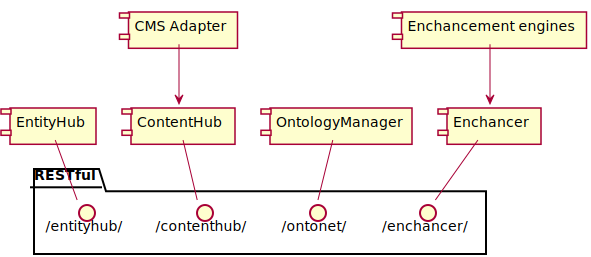
\includegraphics[width=0.6\textwidth]{Bilder/komponenten.png}
\caption{''Komponentendiagramm vom Stanbol''}
\label{fig:komponenten}
\end{figure}

\begin{itemize}
\item \textbf{EntityHub} ist die interne Datenbank, wo die Informationen über Entitäten gespeichert werden. Diese kann sowohl mithilfe von Java API als auch über eine REST-Schnittstelle für die Verlinkung benutzt werden. Als Datenquelle können sowohl ,,Referenced Sites`` (externe Datenquelle die sich auf anderen Maschinen befinden, und auf die EntityHub per Netzwerk zugreift) als auch lokale Indexes verwendet werden. Man kann EntityHub als eine Art von Aggregator betrachten, der mehrere Wissendatenbanke über eine einheitliche API zur Verfügung stellt. 
\item \textbf{Enhancer} und \textbf{EnhancementEngine} sind die Kernkomponenten von Stanbol, die für die Anreicherung von Texten mit Annotationen zuständig sind.
\item \textbf{OntologyManager} wird, wie sagt der Name, für die Verwaltung von Ontologien zuständig.
\item \textbf{ContentHub} wird für die Integration mit CMS gebraucht und stellt eine Datenbank für das \textit{Content} einer CMS zur Verfügung (nicht für die Entitäten!).
\end{itemize}
Im Rahmen dieser Arbeit werden nur Engines und EntityHub gebraucht, andere Module sind für die Extraktion von Entitäten irrelevant.

\paragraph{}
Die grundlegende Idee, die die Architektur von Stanbol prägt, heißt ,,Pipelining`` - ein Fließband, das mehrere Textverarbeitungsschritte miteinander verknüpft, und eine flexible Konfiguration von Kontentanreicherung ermöglicht. Jedes Element dieses Fließbandes wird ,,Engine`` genannt. Von dem Blickwinkel der Architektur wird jedes Engine als selbstständiges BlackBox implementiert, der am Eingang den Text, der angereichert werden soll, mit den von anderen Engines hinzugefügten Annotationen zusammen, bekommt, und am Ausgang neue Annotationen liefert. 

Die Engines werden in sogenannte Ketten zusammengebunden - der Ausgang von einem Engine wird mit dem Eingang von einem anderen Engine verbunden, und so wird eine virtuelle Kette gebaut. Das erste Element in dieser Kette bekommt dabei als Eingang den Text von dem Benutzer, und der Ausgang des letztes Element wird zu dem Benutzer geschickt. 

Auf der Abbildung \ref{fig:ENGINEPIPELINE} wird die Aufbau der in dieser Arbeit verwendeter Engine-Kette noch einmal grafisch dargestellt.
\begin{figure}[ht]
\centering
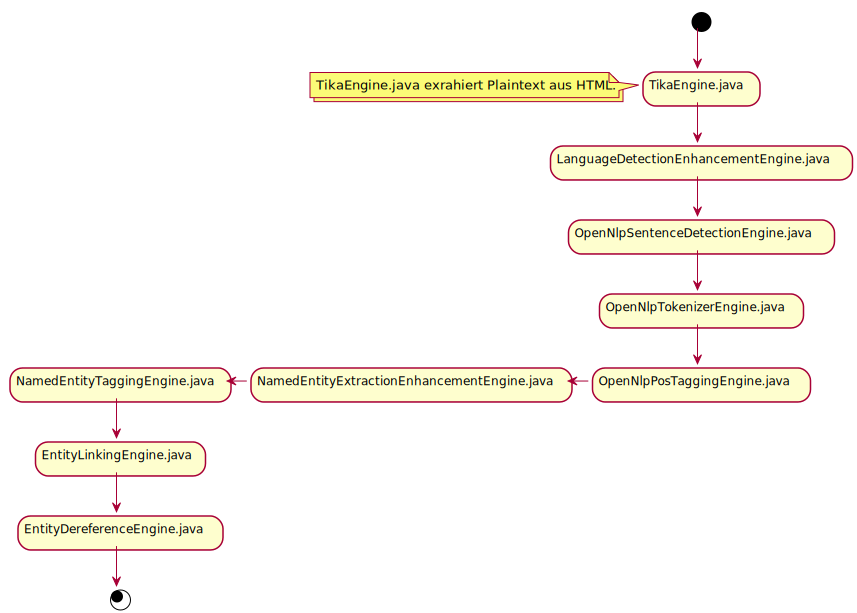
\includegraphics[width=\textwidth]{Bilder/enchancer.png}
\caption{''Graphische Darstellung des Anreicherungspipelines''}
\label{fig:ENGINEPIPELINE}
\end{figure}
Nachdem der Text, der angereichert werden soll, über REST API ausgelesen wurde, werden zuerst rohe Textdaten aus HTML extrahiert, was für Anreicherung von Webseiten notwendig ist. Falls die Daten aber schon im Plaintext gesendet wurden, wird dieser Schritt ignoriert. Danach muss die Sprache des Textes erkannt werden, anhand deren entschieden wird, ob der Text angereichert werden kann. Für die Erkennung der Sprache stellt Stanbol bereits ein Engine \footnote{\url{https://stanbol.apache.org/docs/trunk/components/enhancer/engines/langidengine.html}} zur Verfügung.

Falls die Sprache von der Kette unterstützt wird, werden die Sätze und Tokens extrahiert. Die Engines für Satz- und Tokenserkennung, die auch deutsche Sprache unterstützen, sind als Standardteil der API auch verfügbar.

Anschließend können aus dem Text, der vorberarbeitert wurde, Entitäten extrahiert werden. Nach den Extraktion-, Verlinkung- und Filterungsschritten wird der mit Annotationen angereicherte Text über REST-Schnittstelle zurückgegeben.

Als Entwickler muss man aber gleich beachten, dass die interne Implementierung von Ketten diese Architektur leider nicht anschaulich abbildet. Wie es auf der Abbildung \ref{fig:REALPIPELINE} zu sehen ist, gibt es intern kein Pipeline - stattdessen wird es für jeden Text, der angereichert werden soll, eine Instanz der Data-Klasse ,,ContentItem`` erzeugt, die zwischen allen Engines der Kette geteilt wird. Die Implementierung eines Engines hat technisch gesehen weder Ein- noch Ausgang, und benutzt diese Instanz von ,,ContentItem``, um die Informationen mit anderen Engines auszutauschen. Die Reihenfolge von Elementen in der Engine-Kette bestimmt deswegen eigentlich nicht, wie die Ein- und Ausgänge von Engines verbunden werden sollen, sondern die Reihenfolge, in der die ausgeführt werden müssen.

\begin{figure}[ht]
\centering
\includegraphics[width=\textwidth]{Bilder/realarch.png}
\caption{''Interne Implementierung einer Engine-Kette''}
\label{fig:REALPIPELINE}
\end{figure}
Der Nachteil solcher Architektur ist, dass mehrere Engines unter Umständen auf dieselbe Instanz von ,,ContentItem`` \textbf{gleichzeitig} zugreifen können, was bei Schreibzugriffen zur Beschädigung von Daten führen kann. Deswegen soll jedes Engine die Instanz von ,,ContentItem`` während des Schreibzugriffs sperren lassen.

\section{Extraktion von Entitäten} \label{sec:extraktimpl}
Da die Vorverarbeitungsschritte bereits als Teil von Stanbol implementiert sind, ist die Erkennung von Entitäten das erste Modul, das entwickelt werden muss. Die Schritte, die für die Entwicklung eines Engines unternommen werden müssen, lassen sich wie folgt definieren:
\begin{itemize}
\item Ein Engine wird als ein Objekt der Klasse ,,AbstractEnhancementEngine`` implementiert. 
\item Diese Klasse soll dem Framework folgende Methoden zur Verfügung stellen, die die Integration des Engines in eine Enginekette ermöglichen:
\begin{itemize}
\item Aktivierungsmethode, die ein mal beim Starten des Engines aufgerufen wird. Diese Methode soll das für das Engine benötigte Modell aus einer Datei laden (ein vortraniertes SVM, z.B.).
\item Die Methode, die für den angegebenen Text sagt, ob das Engine diesen Text anreichern kann. Dadurch wird sichergestellt, dass nur die Sprache, die ENgine tatsächlich versteht, bearbeitet wird.
\item Die Hauptmethode, die für den angegebenen Text Annotationen berechnet.
\end{itemize}
\item Die Ketten, die Engines miteinander verbinden, können sowohl während der Laufzeit als auch vor dem Kompilieren des Systems in einer Konfigurationsdatei definiert werden.
\end{itemize}

\subsection{StanfordNER} 
\paragraph{}
Die erste Anreicherungskette wurde auf Basis von StanfordNER\cite{Jenny/etal:07} aufgebaut. Dieses Framework implementiert CRF-Algorithmus und stellt ein Modell für die deutsche Sprache zur Verfügung\cite{faruqui10:_training}. Der Nachteil dieses Engines ist, dass es nur ein vortrainiertes Modell zur Verfügung gestellt wird - das Korpus selbst, auf deren Basis man eigenes Modell trainieren könnte, stehen nicht zur Verfügung. Der Vorteil dabei ist, dass es insgesamt zwei Modellen zur Verfügung stehen:

\begin{enumerate}
\item HGC - Huge German Corpus-generalized classifier - dieses Modell wurde auf Texten aus Zeitungen trainiert.
\item deWac - dieser Klassifikator wurde auf Texten aus Internet trainiert.
\end{enumerate}

Dieses Framework stellt außerdem die Möglichkeit zur Verknüpfung von mehreren Modellen miteinander zur Verfügung. Deswegen kann es im Rahmen dieser Arbeit neben dem Austesten von oben genannten Modellen auch ein kombiniertes Modell getestet werden - es ist möglich, dass ein kombiniertes Modell mehr Entitäten im Text finden könnte, andererseits steigt dabei die Wahrscheinlichkeit von False-Positive-Antworten.

Dieses Framework ist auch für Vorverarbeitung - Zerlegung des Textes in einzelne Sätze und Zerlegung von Sätzen in einzelne Tokens - verantwortlich. Deswegen sind für den auf Stanford-NER basierten Einsatz nur zwei Vorverarbeitung-Engines notwendig:
\begin{enumerate}
\item Tika-Engine für Extraktion von rohen Textdaten aus HTML.
\item Spracherkennungsmodul, mit deren Hilfe sichergestellt wird, dass die Analyse nur für deutsche Sprache gestartet wird.
\end{enumerate}

Die Klassendiagramm für dieses Engine ist auf der Abbildung \ref{fig:stanfclasses} zu sehen.

\begin{figure}[ht]
\centering
\includegraphics[width=\textwidth]{Bilder/stanford-classes.png}
\caption{''Klassendiagramm  des Stanford-Engines''}
\label{fig:stanfclasses}
\end{figure}
\begin{itemize}
\item Die Klasse \textit{StanfordNEREnhancementEngine} ist die Hauptklasse, die nach den Entitäten im Text sucht.
\item \textit{NERClassifierCombiner} ist die interne Klasse des StanfordNER-Frameworks und stellt die Schnittstelle zum Kombinieren von mehreren NER-Modellen zur Verfügung.
\item \textit{NameOccurenceUtility} ist eine Hilfsklasse, die die Daten zwischen StanfordNER- und Stanbol-Format umwandelt.
\item \textit{StanfordTextAnnotationService} ist ein Hilfsservice, das die vom Engine gefundene Entitäten	zum ,,ContentItem`` als Annotationen hinzufügt.
\end{itemize}

\subsection{OpenNLP}
%Beschreibung des OpenNLP-Einsatzes.
Das weitere Algorithmus, das im Rahmen dieser Arbeit verwendet werden soll, ist MaximumEntropy. Es ist als Teil von OpenNLP\footnote{\url{http://opennlp.apache.org/}}-API implementiert. OpenNLP ist ein quelltextoffenes Framework für maschinelle Sprachverarbeitung. Das Framework ist genau wie Stanbol modular aufgebaut, und stellt folgende Funktionalität zur Verfügung:

\begin{itemize}
\item Erkennung von Sätzen. Genau wie für die Extraktion von Entitäten wird für die Satzerkennung ein Maximum-Entropy-Modell verwendet, das vorher trainiert werden muss. Ein Modell für die deutsche Sprache, trainiert auf der Basis von TIGER-Korpus, der in nachfolgendem Kapitel beschrieben ist, ist aber bereits ein Teil des Frameworkes.
\item Zerlegung von Sätzen in Tokens:
\begin{itemize}
\item Die Zerlegung ohne Modell, nur anhand in dem Text vorhandenen Leerzeichen erfolgen. Diese Methode soll aber nicht verwendet werden, da die Fehlerwahrscheinlichkeit zu groß ist.
\item Es kann ein ME-Modell verwendet werden, um Tokens zu erkennen. Der Nachteil dieser Methode ist, dass das Modell zuerst trainiert werden soll, wozu ein Korpus gebraucht wird.
\end{itemize}
\item POS-Tagging - die Erkennung und Annotierung von Wortarten - während dieses Vorgangs wird jedem Token eine entsprechende Wortart zugeordnet.
\item Erkennung von Entitäten.
\end{itemize}

Der Vorteil dieses Engines ist, dass es schon als Teil von Stanbol dem Entwickler zur Verfügung stellt, und so muss nicht neu entwickelt werden. Allerdings müssen für die Extraktion von deutschsprachigen Entitäten die entsprechende ME-Modelle trainiert werden, worauf in der Sektion \ref{subsec:decor} angegangen wird.

Die Klassendiagramm für OpenNLP-Engine ist auf der Abbildung \ref{fig:onlpuml} definiert. Es werden insgesamt nur drei Klassen verwendet:
\begin{itemize}
\item Basisklasse \textit{NEREngineCore}, die die Extraktion von Entitäten mithilfe von ME-Algorithmus implementiert.
\item Die Klasse \textit{CustomNERModelEnhancementEngine}, die von der Basisklasse erbt, und für Behandlung von benutzerdefinierten Modellen zuständig ist.
\item Die Konfigurationsklasse \textit{NEREngineConfig}.
\end{itemize}

\begin{figure}[ht]
\centering
\includegraphics[width=\textwidth]{Bilder/onlp-classes.png}
\caption{''Klassendiagramm  des OpenNLP-Engines''}
\label{fig:onlpuml}
\end{figure}

\subsection{MITIE}
\paragraph{}
Der Einsatz, das implementiert werden soll, ist SVM-Algorithmus. Als Basis wurde für diese Arbeit MITIE\footnote{\url{https://github.com/mit-nlp/MITIE}}-Framework ausgewählt. MITIE steht für ,,MIT Information Extraction`` - ein Framework zur Extraktion von Entitäten und zur Erkennung von binären Relationen. Wie erwähnt, verwendet dieses Framework SVM als Basisalgorithmus für Erkennung von Entitäten, und soll deswegen auch bessere Ergebnisse als OpenNLP oder StanfordNER zeigen können.

\paragraph{Vor- und Nachteile}
\begin{itemize}
\item Vorteile des MITIE-Einsatzes:
\begin{enumerate}
\item Höhere Qualität der Extraktion, im Vergleich zu Maximum Entropy oder CRF.
\item Die Geschwindigkeit der Extraktion ist nicht viel kleiner, als die bei anderen Einsätzen.
\end{enumerate}
\item Nachteile des MITIE-Einsatzes:
\begin{enumerate}
\item Die Größe des Modells ist im Vergleich zu ME oder CRF-Modellen relativ hoch(323 Mb im Vergleich zu 3 Mb für ein OpenNLP-Modell)
\item Das Training eines SVM-Modells kann bis auf mehrere Tage dauern.
\item Ein rein technischer Nachteil - die MITIE-Implementierung ist in C++ geschrieben und ist außerdem nicht thread-sicher, was zu folgenden Einschränkungen führt:
\begin{enumerate}
\item Der Aufruf des Engines muss mit einem Lock gesichert werden, was die Geschwindigkeit bei mehreren gleichzeitigen Benutzer beeinträchtigt.
\item Jeder Fehler in dem Engine kann potentiell zum Absturz der ganzen JVM-Software führen.
\end{enumerate}
\end{enumerate}
\end{itemize}

Die Aufbau dieses Engines ähnelt sich der vom Stanford-NER-Engine, und kann auf der Abbildung \ref{fig:mitieclasses} betrachtet werden.

\begin{figure}[ht]
\centering
\includegraphics[width=\textwidth]{Bilder/mitie-classes.png}
\caption{''Klassendiagramm  des MITIE-Engines''}
\label{fig:onlpuml}
\end{figure}

\subsection{Deutcshe Korpora} \label{subsec:decor}
Nachdem die Engines, die nach Entitäten in Texten suchen sollen, entwickelt wurden, müssen die entsprechende NER-Modelle trainiert werden, wie es in der Sektion \ref{sec:trcorpora} beschrieben wurde. Und obwohl fällt dieser Schritt fürs auf Stanford-NER basierten Engine komplett aus, da dort ein vortrainiertes Modell verwendet wird, muss für weitere zwei Engines eigene Modelle trainiert werden.

Im Rahmen dieser Arbeit wurden zwei Trainingskoprora verwendet: von den Linguisten erzeugtes TIGER-Korpus und aus Basis von Wikipedia-Artikeln aufgebautes PIG-Korpus.

Für Training von Modellen für beide Engines (MITIE und OpenNLP) wird dasselbe Datenformat verwendet, das in der Auflistung \ref{lst:TIGEROPENBEISPIEL} beschrieben ist. Dadurch wird erreicht, dass der Code fürs Training von beiden Engines wiederverwendet werden kann.

\lstinputlisting[captionpos=b,label={lst:TIGEROPENBEISPIEL},caption={Ausschnitt aus einem Korpus im OpenNLP-Format.}]{Listings/tiger-opennlp.txt}

\subsubsection{TIGER Korpus}
\paragraph{}
TIGER-Korpus wurde von dem Institut für Maschinelle Sprachverarbeitung\cite{brants2004tiger} auf der Basis von Zeitungen aufgebaut, und beinhaltet 50474 Sätzen. Außer markierten Entitäten beinhaltet dieser Korpus auch die Informationen über POS (Part Of Speech - ob das Wort ein Verb oder ein Substantiv ist), Lemma (Infinitiv für Verben oder Nominativ Singular für Substantive) und andere Informationen über die annotierte Tokens, wie Kasus oder Genus. Der Ausschnitt des Korpuses findet man in der Auflistung \ref{lst:TIGERBEISPIEL}.

\lstinputlisting[captionpos=b,label={lst:TIGERBEISPIEL},caption={Ausschnitt aus dem TIGER-Korpus. Die Informationen, die in dieser Arbeit nicht gebraucht werden, wurden wegen Platzmangel weggelassen.}]{Listings/tiger-example.txt}
Jeder Satz ist dabei auf einer getrennter Zeile gespeichert, die Tokens werden mit Leerzeichen getrennt, und mithilfe von HTML-ähnlichen Tags werden die Entitäten markiert.

\paragraph{}
Der Korpus ist wie folgt aufgebaut:
\begin{itemize}
\item Die Sätze werden mit einer leeren Zeile getrennt.
\item Jeder Token und seine Annotationen werden in einer Zeile geschrieben. Die Spalten werden mit einem Leerzeichen getrennt.
\item Die erste Spalte beinhaltet ID des Tokens, die aus Nummer des Satzes und Nummer des Tokens innerhalb des Satzes besteht.
\item Die zweite Spalte ist der Token selbst, so wie er auch im Satz vorkommt.
\item In der dritten Spalte steht Lemma des Tokens.
\item Die vierte Spalte wird nicht verwendet.
\item Und die fünfte Spalte beinhaltet POS-Tag des Tokens. Falls dieser Tag den Typ \textit{NE} hat, ist das eine Entität.
\end{itemize}

Der Nachteil dieses Korpuses besteht darin, dass es zwischen verschiedenen Typen von Entitäten nicht unterschieden wird, und die alle den Typ \textit{NE} (NamedEntity) haben.

\paragraph{}
Die Logik, die für die Umwandlung von Tiger Korpuseinträgen in OpenNLP-Format verantwortlich ist, ist in der Auflistung \ref{lst:LOGICOFCONVERTER} zu sehen.
\lstinputlisting[captionpos=b,label={lst:LOGICOFCONVERTER},caption={Ausschnitt aus den Quelltexten des Konverters, der die Logik der Umwandlung beschreibt}]{Listings/tiger-to-onlp.java}
Es wird praktisch für jede ununterbrochene Reihenfolge von NE-Merkierungen ein OpenNLP-Tag erzeugt, und alle Wörter, die keine Entitäten sind, werden ohne Umwandlung kopiert.

\subsubsection{Wikipedia-basiertes Korpus}
\paragraph{}
Leider kann man nicht immer einen manuell aufgebauten Korpus verwenden, entweder aus Lizenz- oder Kostengründen. Viele Korpusse sind nur für Forschung frei verfügbar, was bedeutet, dass 
die auf keinen Fall in einem Geschäftsprojekt verwendet werden dürfen. Und einen eigenen Korpus aufzubauen ist auch nicht immer möglich, da dazu die Linguisten eingesetzt werden müssen, die nicht jede Firma zur Verfügung hat, und es kann Monaten dauern, bis man ein eigenes Korpus erstellt. Was könnte in diesem Fall unternommen werden?

\paragraph{}
Oliver Grisel\footnote{\url{http://www.nuxeo.com/blog/mining-wikipedia-with-hadoop-and-pig-for-natural-language-processing/}} hat einen interessanten Einsatz zur automatischer Aufbau von Korpus vorgeschlagen. Es wird vorgeschlagen, Wikipedia als Textbasis zu nehmen, und die interne Links, die auf andere Wikipediaseiten führen, sollen als  Entitäten markiert werden. Es soll anschließlich ein Korpus aufgebaut werden, auf dessen Basis ein NER-Modell trainiert werden kann. Da Wikipedia auch auf deutscher Sprache verfügbar ist, soll dieser Einsatz auch für Zwecke dieser Arbeit nützlich sein.

\paragraph{}
Um den Korpus aufzubauen, wird Apache Pig\footnote{\url{http://pig.apache.org/}} verwendet - ein Framework für Big-Data-Analyse, der eine Skript-Sprache und JavaAPI zur Verfügung stellt. Die Aufbau vom Korpus umfasst folgende Schritte:
\begin{enumerate}
\item Es wird Dump von Wikipediaartikeln heruntergeladen.
\item Es werden die Listen von Wikipedia-Links und Typen von Entitäten von DBpedia heruntergeladen. Diese Informationen braucht man später, um jeder Entität in dem erzeugten Korpus die richtige Entitätstyp zuordnen zu können.
\item Es werden Links auf interne Wikipedia-Artikeln aus Wikipedia-Dump extrahiert, mit der Positionsinformation zusammen.
\item Jeder Link wird mithilfe von DBpedia-Daten einen Entitätstyp zugeordnet.
\item Es wird ein Trainingskorpus im OpenNLP-Format erzeugt.
\end{enumerate}

\paragraph{} 
Für Korpusaufbau aus deutscher Wikipedia können im Prinzip die Scripts von Oliver Grisel genommen werden, die allerdings angepasst werden müssen:
\begin{itemize}
\item Es soll deutsche Dbpedia, und nicht englische verwendet werden.
\item Es soll deutsches Modell für Satzerkennung anstatt englisches eingesetzt werden.
\item Herunterladen von Wikipedia- und Dbpediadaten soll automatisiert werden.
\end{itemize}

Der Code, der für die Erzeugung eines Wikipedia-basierten Korpus verantwortlich ist, ist in der Auflistung \ref{app:pigcorpus} repräsentiert.

\paragraph{}
Aber welche Vor- und Nachteile hat automatische Erzeugung vom Korpus? Kann das trainierte Modell später auch tatsächlich für sinnvolle Entitätserkennung eingesetzt werden?
\begin{itemize}
\item Vorteile
\begin{itemize}
\item Die Erzeugung von Korpus braucht höchstens eine Stunde, im Vergleich zu manuell annotierten Korpora.
\item Es werden keine Fachleute gebraucht, um Korpus zu erzeugen.
\end{itemize}
\item Nachteile
\begin{itemize}
\item Nicht alle interne Links stellen eine Entität dar, und nicht alle Entitäten sind ein Link - als Folge ist die Qualität des Korpusses deutlich niedriger, als die von manuell aufgebauten.
\item Eine sehr niedrige Varianz - alle Wikipediaartikel sind mehr oder weniger in gleicher Sprache geschrieben, was bedeutet, dass wenn man dem trainierten Modell einen Text zeigt, der sich von einem durchschnittlichen Wikipedia-Artikel deutlich unterscheidet, werden da höchstwahrscheinlich keine Entitäten gefunden.
\end{itemize}
\end{itemize}

\subsection{Training von Modellen}
Sowohl für OpenNLP als auch für MITIE wird Training von Modellen außerhalb von Stanbol durchgeführt. Die Ergebnisse werden dabei in den binären Dateien serialisiert, und später von entsprechenden Engines innerhalb von Stanbol geladen. Der Grund, warum es so gemacht wurde, ist die Geschwindigkeit des Trainings - wie erwähnt, erfordert Training üblich viel größere Rechnerkapazitäten als die Verwendung von Modellen selbst, bei MITIE-Engine sind das mindestens 24 GB RAM, und Training dauert aber trotzdem bis auf eine Woche. Deswegen wurde Training auf getrennten Rechnern durchgeführt.

Die Implementierung von Training an sich selbst ist relativ einfach: 
\begin{enumerate}
\item Zuerst wird die vorab erzeugte OpenNLP-Training-Datei geladen.
\item Danach wird entweder OpenNLP- oder MITIE-API aufgerufen, um ein ME- oder SVM-Modell darauf zu trainieren.
\item Am Ende wird das erzeugte Modell serialisiert und in einer Datei gespeichert.
\end{enumerate}
Das Training von einem OpenNLP-Modell ist in der Auflistung \ref{app:trainonlp} und vom MITIE-Modell in der Auflistung \ref{app:trainmitie} beschrieben.

\section{Verlinkung und Dereferinzierung von annotierten Entitäten}
\paragraph{}
Nachdem die Entitätserkennung durchgeführt wurde, hat man die Informationen darüber, ob es Entitäten im Text gefunden wurden, die Position der Entität innerhalb des Satzes und optional den Typ der Entität. Die Ontologie selbst, die Endbenutzer zu sehen braucht, fehlt allerdings noch. Es müssen noch zwei Schritte durchgeführt werden, bis die Informationen komplett sind - Verlinkung von gefundenen Entitäten mit der Entitäten in DBpedia (oder einer anderer Wissendatenbank) und die Dereferinzierung von Eigenschaften der Entität.

Während der Verlinkung von Entitäten wird für jede erkannte Entität eine Suche nach dieser Entität in einer oder mehreren Wissendatenbanken durchgeführt. Um den Vorgang höchstmöglich zu beschleunigen, soll lokaler Wissendatenbankindex (EntityHub in Terminologie von Stanbol) eingesetzt werden. Dieser Index soll vorher aufgebaut werden, und zumindest die Namen der Entitäten beinhalten. Für spätere Schritte ist aber empfehlenswert, auch diverse Eigenschaften von Entitäten zum Index hinzuzufügen, damit Dereferinzierungschritt auch so schnell wie möglich ausgeführt wird. Es muss aber beachtet werden, dass Index von realen Wissendatenbanken wie DBpedia mehr als 20 Gigabytes wiegen kann, und die Aufbau kann mehrere Tagen in Anspruch nehmen.

Für die Verlinkung von Entitäten wird Engine ,,EntityLinkingEngine`` verwendet, dessen Aufbau auf der Abbildung \ref{fig:linking} beschrieben ist.

\begin{figure}[ht]
\centering
\includegraphics[width=\textwidth]{Bilder/classes-linking.png}
\caption{''UML-Klassendiagramm für EntityLinkingEngine''}
\label{fig:linking}
\end{figure}

Bei der Verlinkung von Entitäten kommt es oft vor, dass die Entitäten, die gefunden wurden, eigentlich nur Verlinkungen auf andere Entitäten, und keine selbstständige Objekten sind - z.B. die Entität ,,CDU`` ist nur ein Link auf ,,Christlich Demokratische Union Deutschlands`` ist. Solche Entitäten werden während der Verlinkung anhand der Eigenschaft ,,dbo:wikiPageWikiLink`` erkannt, und anstatt dieser Zwischenentität wird als Ergebnis der Verlinkung die referenzierende Entität verwendet.

Um die für den Benutzer relevante Informationen (Eigenschaften von Entitäten) zur Verfügung stellen zu können, müssen diese Eigenschaften aus der Datenbank geladen werden. Dazu könnte man auch direkt auf die entsprechende Schnittstelle zugreifen (http://de.dbpedia.org/resource/ für DBpedia, zum Beispiel), so ein Vorgehen würde aber zeitaufwändig und ineffektiv sein. Deswegen soll auch für die Dereferinzierung EntityHub eingesetzt werden. Für diesen Zweck wird Engine \textit{EntityhubDereferenceEngine} eingesetzt, der für jede im Verlinkungsschritt gefundene Entität alle für den Link verfügbare Eigenschaften zu dem Anreicherungsergebnis hinzufügt.

Als Wissendatenbank für die Verlinkung und Dereferinzierung wird in dieser Arbeit lokaler Index von deutscher DBpedia\cite{auer2007dbpedia} verwendet. DBPedia stellt eine Kopie von Wikipedia zur Verfügung, deren Daten als RDF-Graphen gespeichert werden, und auf die mithilfe von SPARQL zugegriffen werden kann.

\subsection{Rausfielterung von für den Benutzer irrelevanten Entitäten}

\section{API f{\"{u}}r Anreicherung von Suchergebnissen}
\paragraph{}
Um dem Endentwickler die Anreicherung von Suchergebnissen so einfach wie möglich zu machen, wurde eine API entwickelt, die man direkt an sein Projekt als eine Bibliothek anbinden kann. Diese Bibliothek wird auch später in der Evaluierung verwendet. Es wird eine Abstraktionsschicht hinzugefügt, die die Aufrufe der REST-Schnittstelle von Stanbol hinter der Klientklasse verbirgt. Der Entwickler soll nur die Liste von Suchsnippets an API übergeben, für die Verbindungaufbau zum Stanbol und Parsing der Antwort des Servers ist API verantwortlich. Die Beschreibung der API-Schnittstelle findet man in der Auflistung \ref{lst:APISCHNITSTELLE}. 

\lstset{language=Java}
\lstinputlisting[captionpos=b,label={lst:APISCHNITSTELLE},caption={Die API-Schnittstelle zum Stanbol}]{Listings/api.txt}

Als Eingabedaten übergibt man die Liste von URLs gefundenen Webseiten mit dazugehörigen Texten von Snippets zusammen, und als Ausgabe bekommt man für jede URL die Liste von gefundenen Entitäten. Da in Rahmen dieser Arbeit mehr verschiedenen Engineketten implementiert wurden, muss der Name der erwünschten Kette miteingegeben werden.
\chapter{Evaluierung}

\section{Benutzerevaluierung}
\paragraph{}
Damit es festgestellt werden könnte, ob die Anreicherung von Suchergebnissen mit aus den Snippets extrahierten Entitäten für den Benutzer auch tatsächlich hilfreich sein könnte, wurde eine Benutzerevaluierung durchgeführt. Die Evaluierung sollte folgende Fragen beantworten:

\begin{itemize}
\item Welcher Einsatz liefert dem Benutzer die zu der Anfrage am besten passende Entitäten? 
\item Wird die Geschwindigkeit der Suche durch zusätzlicher Schritt der Extraktion von Entitäten stark beeinträchtigt? Ist die Beeinträchtigung der Geschwindigkeit groß Genug, um den Benutzer bei der Suche zu stören?
\item Gibt es Korrelationen zwischen ,,standarten`` Metriken wie F-Measure und Precision/Recall und der Zufriedenheit der Benutzer, oder kann man aus der rein numerischen Metriken keine Aussage treffen, ob der Engine in der Lage ist, eine genügende Benutzerunterstützung zu leisten?
\end{itemize}

Um diese Fragen beantworten zu können, wurde eine Webseite aufgebaut, die dem Benutzer die Möglichkeit gibt, alle Engines und alle Modellen, die im Rahmen dieser Arbeit verwendet wurden, zu bewerten. Insgesamt kann der Evaluirungsvorgang in drei Schritten geteilt werden:

\begin{enumerate}
\item In dem Einleitungsschritt wird dem Benutzer erklärt, wie genau die Evaluierung abläuft, und was wir von ihm brauchen.
\item Danach muss der Benutzer alle vorhandene Kombinationen von Modellen und Engines bewerten. Dazu soll eine Frage aus der vorgegebenen Liste ausgewählt und gestellt werden, die zuerst an Bing gesendet wird, und dann an unseres Stanbol-Backend.
\item Um die Situation, wo der Benutzer sich ,,betrogen`` fühlen könnte, möglichst auszuschließen, wird dem Probanden die Möglichkeit gegeben, jede beliebige Frage zu stellen, und dann einen persönlichen schriftlichen Feedback abzugeben.
\end{enumerate}

\begin{figure}
\centering
\includegraphics[width=1.0\textwidth]{Bilder/evalstep1.png}
\caption{''Einleitung in die Evaluierung''}
\label{fig:evalstep01}
\end{figure}

\begin{figure}
\centering
\includegraphics[width=1.0\textwidth]{Bilder/evalstep2.png}
\caption{''Bewertung eines Engines''}
\label{fig:evalstep01}
\end{figure}

\begin{figure}
\centering
\includegraphics[width=1.0\textwidth]{Bilder/evalstep3.png}
\caption{''Der letzte Schritt der Evaluierung''}
\label{fig:evalstep01}
\end{figure}

\section{Zusammenfassung}
Erkenntnissen aus der Studie und den Konsequenzen für die Arbeit.
%\chapter{Zusammenfassung}


\section{Zusammenfassung}
Was genau haben wir erreichen können? Ist der Einsatz erfolgreich? Was könnte verbessert werden? Wirtschaftliche Perspektiven - 

\section{Diskussion}


\section{Ausblick}



% Anhang
%\cleardoublepage
%\pagenumbering{roman}
%\part*{Anhang}
%\begin{appendix}
%\chapter{Listings}

\lstset{language=Java}
\lstinputlisting[captionpos=b,label={app:feedbacks},caption={Die Liste von Benutzerfeedbacks}]{Listings/feedbacks.json}

\lstset{language=Java}
\lstinputlisting[captionpos=b,label={app:pigcorpus},caption={Erzeugung eines Wikipedia-Korpus}]{Listings/pig.java}

\lstset{language=Java}
\lstinputlisting[captionpos=b,label={app:trainonlp},caption={Training eines ME-Modells (OpenNLP)}]{Listings/train-onlp.java}

\lstset{language=python}
\lstinputlisting[captionpos=b,label={app:trainmitie},caption={Training eines ME-Modells (OpenNLP)}]{Listings/train-mitie.py}

\lstset{language=Java}
\lstinputlisting[captionpos=b,label={lst:APISCHNITSTELLE},caption={Die API-Schnittstelle zum Stanbol}]{Listings/api.txt}

%\clearpage
%\chapter{Tabellen}

\clearpage
\chapter{Screenshots}

\begin{figure}
\centering
\includegraphics[width=1.0\textwidth]{Bilder/evalstep01.png}
\caption{''Einleitung in die Evaluierung''}
\label{app:evalstep01}
\end{figure}

\begin{figure}
\centering
\includegraphics[width=.6\textwidth]{Bilder/select-question.png}
\caption{''Auswahl einer Frage''}
\label{fig:eval-select-question}
\end{figure}

\begin{figure}
\centering
\includegraphics[width=1\textwidth]{Bilder/evalstep02-step1.png}
\includegraphics[width=0.5\textwidth]{Bilder/evalstep02-step1-2.png}
\caption{''Liste von Snippets und gefundenen Entitäten''}
\label{fig:eval-entitylist}
\end{figure}

\begin{figure}
\centering
\includegraphics[width=1\textwidth]{Bilder/eval-step03.png}
\caption{''Liste von Eigenschaften einer Entität''}
\label{fig:eval-props}
\end{figure}

\begin{figure}
\centering
\includegraphics[width=0.6\textwidth]{Bilder/bewertung-eval.png}
\caption{''Bewertung eines Engines''}
\label{fig:bewertung}
\end{figure}

\begin{figure}
\centering
\includegraphics[width=0.6\textwidth]{Bilder/ende-eval-01.png}
\caption{''Eingabeform des letzten Evaluierungsschritt''}
\label{fig:finish-eval}
\end{figure}

%\end{appendix}

% Verzeichnisse
\cleardoublepage
\part*{Verzeichnisse}
%\listoffigures
%\listoftables
%\lstlistoflistings
\bibliographystyle{plain}
\bibliography{literatur}

% Erklärung
%\cleardoublepage
%\pagestyle{empty}
%\begin{center}
\Large{\textsf{\textbf{Erklärung}}}
\end{center}
\vspace{0.8cm}
Hiermit erkläre ich, dass ich die vorliegende Arbeit ohne fremde Hilfe selbstständig
verfasst und nur die angegebenen Quellen und Hilfsmittel benutzt habe. Ich versichere
weiterhin, dass ich diese Arbeit noch keinem anderen Prüfungsgremium vorgelegt habe.

Duisburg, im November 1492
\\[1cm]
.................................................\\[0.2cm]
Manfred Mustermann
%\pagestyle{empty}
%\cleardoubleemptypage

\end{document}
